\documentclass[lettersize,journal]{IEEEtran}
\usepackage{amsmath,amsfonts}
\usepackage{algorithmic}
\usepackage{algorithm}
\usepackage{array}
\usepackage[caption=false,font=normalsize,labelfont=sf,textfont=sf]{subfig}
\usepackage{textcomp}
\usepackage{stfloats}
\usepackage{url}
\usepackage{verbatim}
\usepackage{graphicx}
\usepackage{cite}
\hyphenation{op-tical net-works semi-conduc-tor IEEE-Xplore}
% updated with editorial comments 8/9/2021

% \usepackage{amsmath,amsfonts}
% \usepackage{algorithmic}
% \usepackage{array}
% \usepackage[caption=false,font=normalsize,labelfont=sf,textfont=sf]{subfig}
% \usepackage{cite}
% \usepackage{textcomp}
% \usepackage{stfloats}
% \usepackage{url}
% \usepackage{verbatim}
% \usepackage{graphicx}
\usepackage{amssymb}
\usepackage{xcolor}
% \usepackage{appendix}
% \usepackage{algorithm}
\usepackage{amsthm}
% \usepackage{multirow} 
% \usepackage{multicol} 
% \usepackage{color}
\usepackage{bm}
% \hyphenation{op-tical net-works semi-conduc-tor IEEE-Xplore}
\usepackage{hyperref}
\usepackage{scalerel}
\usepackage{float}%提供float浮动环境
\usepackage{booktabs}%提供命令\toprule、\midrule、\bottomrule
\newtheoremstyle{custom}
  {\topsep}    % 上方间距
  {\topsep}    % 下方间距
  {\normalfont} % 定理内容的字体 (普通字体)
  {1em}           % 缩进量
  {\itshape}   % 定理标题的字体 (斜体)
  {:}          % 标题后的标点符号
  { }          % 标题后与内容的间距
  {\thmname{\textit{#1}}% 定理标题格式 (斜体)
   \thmnumber{ \textit{#2}}% 定理编号格式 (斜体)
   \thmnote{ \textit{(#3)}}}% 定理备注格式 (斜体)
% 应用自定义样式
\theoremstyle{custom}
\newtheorem{Thm}{Theorem}
\newtheorem{Lem}{Lemma}
\newtheorem{Cor}{Corollary}
\newtheorem{Def}{Definition}
\newtheorem{Exam}{Example}
\newtheorem{Alg}{Algorithm}
\newtheorem{Prob}{Problem}
\newtheorem{subproblem}{Problem}[Prob]
\newtheorem{Rem}{Remark}
\newcommand{\RNum}[1]{\uppercase\expandafter{\romannumeral #1\relax}}
\newcommand{\tabincell}[2]{\begin{tabular}{@{}#1@{}}#2\end{tabular}}
% \theoremseparator{:}
\newtheorem{hyp}{Hypothesis}

\begin{document}

\title{A TREE Oriented Embodied AI Multiplexing Framework for Green 6G Networks}

\author{IEEE Publication Technology,~\IEEEmembership{Staff,~IEEE,}
        % <-this % stops a space
\thanks{This paper was produced by the IEEE Publication Technology Group. They are in Piscataway, NJ.}% <-this % stops a space
\thanks{Manuscript received April 19, 2021; revised August 16, 2021.}}

% The paper headers
\markboth{Journal of \LaTeX\ Class Files,~Vol.~14, No.~8, August~2021}%
{Shell \MakeLowercase{\textit{et al.}}: A Sample Article Using IEEEtran.cls for IEEE Journals}

\IEEEpubid{0000--0000/00\$00.00~\copyright~2021 IEEE}
% Remember, if you use this you must call \IEEEpubidadjcol in the second
% column for its text to clear the IEEEpubid mark.

\maketitle

\begin{abstract}
This document describes the most common article elements and how to use the IEEEtran class with \LaTeX \ to produce files that are suitable for submission to the IEEE.  IEEEtran can produce conference, journal, and technical note (correspondence) papers with a suitable choice of class options. 
\end{abstract}

\begin{IEEEkeywords}
Article submission, IEEE, IEEEtran, journal, \LaTeX, paper, template, typesetting.
\end{IEEEkeywords}

\section{Introduction}
\IEEEPARstart{X}{xx}...  
Multi-modal sensor fusion and unstructured environment are identified as two key features of embodied AI \cite{li_developments_2025}. However, xxx. 
Wireless communication is also identified as a crucial enabling technology for embodied robotics, especially humanoid and xxx, for the flexible and ubiquitous characteristics. 

In order to fuse the multi-modal sensory data and adapt into the dynamic unstructured environments, xxx AI-assisted methods have been proposed. In the early researches, xxx. Due to its multi-task emergence abilities, VLA has become a heated research topic. \cite{}, \cite{}, \cite{} performs high-accuracy action inference in a xxx of embodied tasks. However, these architectures overlook xxx, xxx in practical deployments. 

For practical deployment, several architectures are developed to mitigate the xxx. The embodied LAM architectures are mainly divided into 2 architectures, end-to-end VLA and dual system. End-to-end VLA includes xxx, xxx, and xxx. They xxx. However the end-to-end architectures xxx and suffer latency and power consumption draw-backs on humanoid and xxx embodied systems. To mitigate these drawbacks, dual system, including Helix, InternVLA, GR00T, xxx. Although the dual system embodied AI architectures xxx, they still fail to adapt into dynamic and resource limited wireless systems. 

To fill this gap, recent token pruning methods \cite{}, \cite{} manage to reduce token overhead. xxx. WNCS techniques \cite{}, \cite{}, \cite{} are also one of the candidate techniques to xxx. Semantic-aware and goal-oriented methods \cite{}, \cite{}, \cite{} xxx. Despite the corresponding performance improvements spotted in the up-mentioned methods, the fundamental performance bound for hybrid VLA data transmission under wireless links is still uninvestigated. 

Motivated by these, our main contributions are summarized as follows: 
\begin{itemize}
    \item \bf{xxx} xxx. 
    \item \bf{xxx} xxx. 
    \item \bf{xxx} xxx. 
\end{itemize}

And the rest of the paper are organized as follows. xxx. 

\section{System Model}
In this paper, we study a wireless-enabled embodied AI (WEEA) system, where an embodied agent and the corresponding sensing nodes $\mathcal{S} = \{1, \ldots, s, \ldots, S\}$ are connected to the edge remote controller $e$ with Vision-Language-Action (VLA) equipped. 
% $I$ agents with sensing and action abilities are distributed in the space. 
The system is illustrated in Fig.~\ref{}. Each sensing node perceives the environment with observations $\mathcal{V}_s(t) \in \mathcal{V}(t)$ (e.g., RGB images), its raw data volume is identified with $d_s(t)$. The edge VLA model receive $\mathcal{V}(t)$ and a time-invariant language instruction (prompt) $p$, then predict an action sequence $\mathcal{A}(t)$ (e.g., end-effector poses or joint velocities), $\Pi_\theta(\mathcal{A}(t) \vert \mathcal{V}(t), p)$, where $\theta$ denotes the VLA model parameter. 
% singel-cell system where the base station (BS) is equipped with edge computing power, serving a set of user equipments (UEs), denoted by $i \in \mathcal{I}$. 
% Each agent contains hybrid content transmissions of multi-modal sensory data from helper agent $j$ to ego agent $i$, denoted with ${\bf d}_{j, i}(t) = \{ d^\mathrm{v}_{j, i}(t), d^\mathrm{r}_{j, i}(t), \ldots \}$, where $d^\mathrm{v}_{j, i}(t)$, $d^\mathrm{r}_{j, i}(t)$ represent the transmission data volume of vision, radar, etc., from helper agent $j$ to ego agent $i$, respectively. 
% Each agent contains hybrid content transmissions of multi-modal sensory data and control data, profiled with ${\bf q}_i(t) = \{ {\bf q}^\mathrm{v}_i(t), {\bf q}^\mathrm{r}_i(t), {\bf q}^\mathrm{ms}_i(t), \ldots , {\bf q}^\mathrm{mc}_i(t) \}$, where ${\bf q}^\mathrm{v}_i(t) = \{ {\bf d}^\mathrm{v}_i(t), f^\mathrm{v} \}$, ${\bf q}^\mathrm{r}_i(t) = \{ {\bf d}^\mathrm{r}_i(t), f^\mathrm{r} \}$, ${\bf q}^\mathrm{ms}_i(t) = \{ d^\mathrm{ms}_i(t), f^\mathrm{ms} \}$ and ${\bf q}^\mathrm{mc}_i(t) = \{ d^\mathrm{mc}_i(t), f^\mathrm{mc} \}$ represent the transmission profile of vision, radar, motor state and motor control for agent $i$, including data volume and transmission frequency, respectively. 


% \subsection{xxx Protocol Design}
% Identifying the multi-modal sensory feedback

% The communication resource grid is 



% Puncturing\footnote{xxx} and finite block-length short packet transmission are enabled for ultra low-latency high-reliability motor state and control signal transmissions. The puncturing duration at sub-channel $f$ is denoted by $t_{i, f} < T_k, i \in \mathcal{I}_{m}$. 
% % Puncturing\footnote{xxx} is enabled for ultra low-latency high-reliability transmissions, which is suitable for text queries transmissions carrying more semantic information within each bits \cite{}. 

\subsection{Communication Model}
The up-link transmission rate from sensing node $s$ to the edge server at slot $t$ is described as
\begin{align}
    r_{s}(t) = B_s(t) log_2\left(1 + \mathrm{SNR}_s \right), \forall s \in \mathcal{S}, 
\end{align}
where $B_s(t)$ and $\mathrm{SNR}_s$ denote the fractional bandwidth allocated to $s$ and the signal-to-noise ratio (SNR) of $s$, respectively. The fractional bandwidth allocation follows
\begin{align}\label{bandwidth_cons}
    \sum_{s \in \mathcal{S}}B_s(t) \leq B, 
\end{align}
where $B$ is the system bandwidth\footnote{We assume that adequate bandwidth $B$ is semi-persistently allocated to the WEEA system via orthogonal radio access network (RAN) slicing techniques \cite{}, \cite{}}. 

% The transmission rate from helper agent $j$ to ego agent $i$ at slot $t$ is described as: 
% \begin{align}
%     r_{j, i}(t, f) = B \sum_{f \in \mathcal{F}} b_{f, j, i}(t) \log_2\left(1 + \frac{p_{j, i}(t) h_{j, i}(t)}{\vartheta^2} \right), 
%     % i \in \mathcal{I}_i \cup \mathcal{I}_v &, 
% \end{align}
% % \begin{align}
% %     r_{n, i}(t, f) = (1 - \sum_{i \in \mathcal{I}_\mathrm{t}}\frac{t_{i, f}}{T_k})\log_2\left(1 + \frac{p_{n, i}(t) h_{n, i}(t)}{\vartheta^2} \right) &, \nonumber\\
% %     i \in \mathcal{I}_i \cup \mathcal{I}_v &, 
% % \end{align}
% where $h_{j, i}(t)$ is the channel coefficient from $j$ to $i$, $B$ is unit bandwidth of sub-channel, $\vartheta$ is the xxx and $b_{f, j, i}(t)$, $p_{j, i}(t)$ is the sub-channel allocation indicator and the transmit power, respectively. $b_{f, j, i}(t) = 1$ means sub-channel $f$ is allocated for the data transmission from $j$ to $i$ and $b_{f, j, i}(t) = 0$ otherwise.  The transmit power of each agent $i$ is bounded by 
% \begin{align}
%     \sum_{i \in \mathcal{I}, i \neq j} p_{j, i}(t) \leq P_\mathrm{max}. 
% \end{align}
% Transmission power consumption \cite{xu_energy-efficient_2013} for each BS $n$ is given as
% \begin{align}
%     P_{n}^{\mathrm{com}} = P_S + \alpha \cdot P_T
% \end{align}
% where $P_S$ and $\alpha$ represents the static circuit power and the power amplification coefficient, respectively. 

\subsection{Top-$k$-enabled Token Compression Model}
% Each edge server cache a set of $\mathcal{L}_n$ LAMs. 
In order to support timely and efficient perceptional data delivery, top-$k$ Token compression techniques are widely investigated \cite{}, \cite{}. 

Through Tokenization and top-$k$ Token pruning, the raw observations $\mathcal{V}_s(t)$ are locally compressed at $s$ in terms of observation feature\footnote{On-device/local Tokenizers and Token pruning Techniques are proved to be applicable and helpful in the area of multi-view VLA systems \cite{}, \cite{}. }, and thus we have the exact air-interface transmission data volume denoted as: 
\begin{align}
    d_s^{k_s}(t) = \frac{\alpha_s k_s}{n_s} d_s(t), \forall s \in \mathcal{S}, 
\end{align}
where $\alpha_s$, $k_s$ and $n_s$ denote the normalized xxx rate for the LAM Tokenizer, the output Token length after top-$k$ token pruning and the original Token length, respectively. We denote the top-$k$ decision variable set as ${\bf k} = \{k_1, \ldots, k_s, \ldots, k_S\}$

With top-$k$ Token compression, the corresponding VLA model in the WEEA system suffers the performance degradation, and the comprehensive VLA output performance in terms of long-term average action mean square error (MSE) \cite{} is denoted by 
\begin{align}
    \epsilon_{\bf k} = \mathbb{E} \left[\sum_{t = 1}^T\vert\vert \mathcal{A}_{\bf k}(\mathcal{V}(t)) - \mathcal{A}^*(\mathcal{V}(t)) \vert\vert^2_2\right], 
\end{align}
where $\mathcal{A}_{\bf k}(\mathcal{V}(t))$ is the perturbed action generated with the pruned multi-view observations. 

% The transmission data volume from helper agent $j$ to ego agent $i$ with top-$k$ Token pruning \cite{} is given by 
% \begin{align}
%     d^\mathrm{v}_{j, i}(t) = \frac{k^\mathrm{v}_{j, i}}{n^\mathrm{v}}D^\mathrm{v}_{j, i}(t), 
% \end{align}
% % where xxx. And the corresponding QoS metrics for each LAM in terms of accuracy and delay are listed as follows
% where ${\bf k} = \{ \{k^\mathrm{v}_{j, i}\}, \{k^\mathrm{r}_{j, i}\}, \ldots \}$ denotes the whole set of top-$k$ Token pruning rate. 

% And the corresponding VLA inference action error requirement of agent $i$ is listed as follows
% \begin{align}\label{accuracy_cons}
%     \epsilon_i({\bf k}, t) \leq \delta_i, \forall i \in \mathcal{I}, 
% \end{align}
% % \begin{align}\label{accuracy_delay_cons}
% % \left\{
% %     \begin{array}{l l}
% %         q() \geq \rho_l, \forall l \in \mathcal{L}_n, \forall n \in \mathcal{N}_{BS}, \\
% %         d() \leq \delta_l, \forall l \in \mathcal{L}_n, \forall n \in \mathcal{N}_{BS}. 
% %     \end{array}
% % \right. 
% % \end{align}
% where $\epsilon_i({\bf k})$ and $\delta_i$ denotes the VLA inference error and error threshold of agent $i$, respectively. 
% % where $\rho_l$ and $\delta_l$ are corresponding accuracy and delay thresholds of LAM $l$. 

% Computing power consumption for each agent $i$ is given according to the well investigated dynamic voltage and frequency scaling (DVFS) \cite{guerreiro_modeling_2019} as follows
% \begin{align}
%     P_{i}^{\mathrm{comp}} = 
% \end{align}

\section{Problem Formulation}
We have the original action error minimization problem given by
\begin{Prob}[Original Action Error Minimization Problem]
    The action error of the WEEA system can be minimized via the following optimization problem. 
    \begin{align}
        \underset{{\bf k}, \{B_s(t)\}}{\textrm{minimize}} \quad\quad & \epsilon_{\bf k} \nonumber\\
        \textrm{subject to} \quad\quad  & r_s(t) \geq d_s^{k_s}(t), \forall s \in \mathcal{S}, \label{rate_cons}\\
        & \eqref{bandwidth_cons}, \nonumber
    \end{align}
    where \eqref{rate_cons} is the up-link transmission rate requirement for top-$k$ compressed feature transmission at $s$. 
\end{Prob}

This problem is generally challenging for the following reasons. 
First, xxx. 
Second, xxx. 
Beyond these, xxx. 

However, by xxx, we can analyze the sensitivity of $k$ under various settings, xxx. 
% To start with, we have the cost-efficiency ratio of the WEEA system denoted as: 
% \begin{align}
%     \eta = 
% \end{align}
% % To start with, we have the cost-efficiency ratio of the embodied LAM system denoted as
% % \begin{align}
% %     \eta_{xxx} = \frac{\sum_{i} \alpha_i({\bf k}, t)}{\sum_j \sum_{i \in \mathcal{I}, i \neq j} p_{j, i}(t) + \sum_{i} P^{comp}_i}, 
% % \end{align}
% % where $\alpha_i({\bf k}, t)$ stands for the xxx. 
% % To start with, we have the token responsive energy-efficiency metric \cite{yu_tree_2026} for the distributed MLAM inference-integrated edge BS system denoted as 
% % \begin{align}
% %     \eta_{TREE} = \frac{\displaystyle\sum_{n \in \mathcal{N}_{BS}}\displaystyle\sum_{l \in \mathcal{L}_n}\beta_l \cdot T_l}{\displaystyle\sum_{n \in \mathcal{N}_{BS}}(P_{n}^{\mathrm{com}} + P_{n}^{\mathrm{comp}})}
% % \end{align}
% % where $\beta_l$ is the normalization factor converting tokens to bit-equivalent utility for cached LAM $l$\footnote{The normalization factor is determined corresponding to the token pricing strategies. For example, xxx, xxx, xxx. \cite{} }. 

% And the original cost-efficiency ratio optimization problem is given by 
% \begin{Prob}[Original Cost-efficiency Ratio Maximization Problem]
%     The cost-efficiency ratio of the xxx system can be maximized via the following optimization problem. 
%     \begin{align}
%         \underset{{\bf k}, \{B_s(t)\}}{\textrm{maximize}} && \eta \nonumber\\
%         \textrm{subject to} && r_s(t) \geq d_s^{k_s}(t), \forall s \in \mathcal{S}, \label{rate_cons}\\
%         && \eqref{bandwidth_cons}
%         % P_i^\mathrm{comp} \leq P_\mathrm{max}^\mathrm{comp}, \forall i \in \mathcal{I}, \label{computational_cons}\\
%         % && P_n^\mathrm{com} \leq P_\mathrm{max}^\mathrm{com}, \forall n \in \mathcal{N}_{BS}, \label{communication_cons}\\
%         % && \eqref{accuracy_cons}, \nonumber
%     \end{align}
% \end{Prob}
\section{Problem Transformation}

\section{Proposed Solutions}

\section{Performance Analysis}

\section{Simulation Results}

\section{Conclusions}

\bibliographystyle{IEEEtranc}
\bibliography{IEEEfull, references} 

% \begin{thebibliography}{1}
% \bibliographystyle{IEEEtran}

% \bibitem{ref1}
% {\it{Mathematics Into Type}}. American Mathematical Society. [Online]. Available: https://www.ams.org/arc/styleguide/mit-2.pdf

% \bibitem{ref2}
% T. W. Chaundy, P. R. Barrett and C. Batey, {\it{The Printing of Mathematics}}. London, U.K., Oxford Univ. Press, 1954.

% \bibitem{ref3}
% F. Mittelbach and M. Goossens, {\it{The \LaTeX Companion}}, 2nd ed. Boston, MA, USA: Pearson, 2004.

% \bibitem{ref4}
% G. Gr\"atzer, {\it{More Math Into LaTeX}}, New York, NY, USA: Springer, 2007.

% \bibitem{ref5}M. Letourneau and J. W. Sharp, {\it{AMS-StyleGuide-online.pdf,}} American Mathematical Society, Providence, RI, USA, [Online]. Available: http://www.ams.org/arc/styleguide/index.html

% \bibitem{ref6}
% H. Sira-Ramirez, ``On the sliding mode control of nonlinear systems,'' \textit{Syst. Control Lett.}, vol. 19, pp. 303--312, 1992.

% \bibitem{ref7}
% A. Levant, ``Exact differentiation of signals with unbounded higher derivatives,''  in \textit{Proc. 45th IEEE Conf. Decis.
% Control}, San Diego, CA, USA, 2006, pp. 5585--5590. DOI: 10.1109/CDC.2006.377165.

% \bibitem{ref8}
% M. Fliess, C. Join, and H. Sira-Ramirez, ``Non-linear estimation is easy,'' \textit{Int. J. Model., Ident. Control}, vol. 4, no. 1, pp. 12--27, 2008.

% \bibitem{ref9}
% R. Ortega, A. Astolfi, G. Bastin, and H. Rodriguez, ``Stabilization of food-chain systems using a port-controlled Hamiltonian description,'' in \textit{Proc. Amer. Control Conf.}, Chicago, IL, USA,
% 2000, pp. 2245--2249.

% \end{thebibliography}


% \newpage

% \section{Biography Section}
% If you have an EPS/PDF photo (graphicx package needed), extra braces are
%  needed around the contents of the optional argument to biography to prevent
%  the LaTeX parser from getting confused when it sees the complicated
%  $\backslash${\tt{includegraphics}} command within an optional argument. (You can create
%  your own custom macro containing the $\backslash${\tt{includegraphics}} command to make things
%  simpler here.)
 
% \vspace{11pt}

% \bf{If you include a photo:}\vspace{-33pt}
% \begin{IEEEbiography}[{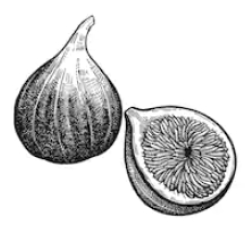
\includegraphics[width=1in,height=1.25in,clip,keepaspectratio]{fig1}}]{Michael Shell}
% Use $\backslash${\tt{begin\{IEEEbiography\}}} and then for the 1st argument use $\backslash${\tt{includegraphics}} to declare and link the author photo.
% Use the author name as the 3rd argument followed by the biography text.
% \end{IEEEbiography}

% \vspace{11pt}

% \bf{If you will not include a photo:}\vspace{-33pt}
% \begin{IEEEbiographynophoto}{John Doe}
% Use $\backslash${\tt{begin\{IEEEbiographynophoto\}}} and the author name as the argument followed by the biography text.
% \end{IEEEbiographynophoto}




\vfill

\end{document}


